\documentclass[a4paper,12pt]{article} % only 10 (default), 11 and 12 pt are available

% NECESSARY PACKAGES
\usepackage[utf8]{inputenc} % to be able to use non-English characters
\usepackage{amsmath}  % improve math presentation
\usepackage{amssymb}
\usepackage{xcolor}
\usepackage{float}
\usepackage{caption} % captioning package of wonders
\usepackage{url} % to incorporate clickable links
\usepackage{cite} % takes care of citations
\usepackage[final]{hyperref} % adds hyper links inside the generated PDF file
\usepackage{placeins}

% NECESSARY FOR INCREASED CUSTOMIZATION PACKAGES
\usepackage{newfloat} % for defining new float in environments (e.g: figure and tables are floats)
\usepackage{graphicx} % takes care of graphic including machinery
\usepackage{tabularx} % extra features for tabular environment
\usepackage{array} % provides 'programmable' tables (cells can be tweaked much more)
\usepackage[export]{adjustbox} % to include boxed content other than figures (e.g: boxed equations)
\usepackage{wrapfig} % to make figures wrap around text
\usepackage{subcaption} % to make sub-figures inside of figures

% TWEAKS FOR PACKAGES
\usepackage[margin=2.54cm,a4paper]{geometry} % tweaks margins
\captionsetup{justification=centering} % caption justification
\captionsetup{font=12pt} % caption text size
\captionsetup{labelfont=bf} % caption label font emphasis (e.g: 'Figure X:')
\numberwithin{equation}{section} % equations are named according to their section (e.g: 2.1)
\numberwithin{figure}{section} % figures are named according to their section (e.g: 3.4)
\hypersetup{
    colorlinks=true,      % false: boxed links; true: colored links
    linkcolor=black,      % color of internal links
    citecolor=blue,       % color of links to bibliography
    filecolor=magenta,    % color of file links
    urlcolor=red          % color of website links
}

\usepackage{lipsum} % DELETE THIS AND BELOW \lipsum[]'s AND YOU'RE GOOD TO GO

%++++++++++++++++++++++++++++++++++++++++++++++++++++++++++++++++++++++++++++++++

% HERE GOES THE COVER PAGE SETUP
\newcommand{\hwcourse}{\text{Progress Report}} % Title of your document
\newcommand{\hwnumber}{\text{PHYS 3266}} % Name of your study number
\newcommand{\hwdetails}{ \text{Simulating Orbital Perturbations and Inferring their Sources} \\ }
\newcommand{\hwauthor}{-Joshua Brandt- \\
                        -Paul Vollrath-  \\
                        -Chloe Fair- } % Your name or your group's names
\newcommand{\HRule}{\rule{\linewidth}{0.5mm}} % line widths in the cover page


%++++++++++++++++++++++++++++++++++++++++++++++++++++++++++++++++++++++++++++++++

\begin{document}

% COVER PAGE IS COMPILED HERE
\begin{titlepage}

\begin{center} % Center remainder of the page
% LOGO SECTION
\includegraphics[width = 8cm]{SoPBanner.jpeg}

\\[2cm]

% HEADING SECTIONS
\textsc{\LARGE Georgia Institute of Technology}\\[.5cm]
\textsc{\Large School of Physics}\\[1.5cm]

% TITLE SECTION
\HRule \\[0.4cm]
{ \huge \bfseries \hwcourse}\\ \vspace{.5cm}
{ \huge \bfseries \hwnumber}\\ \vspace{.5cm}
{ \large \bfseries \hwname}\\ \vspace{.5cm}
{ \hwdetails}\\ \vspace{.5cm}
{ \bfseries \hwdate}\\ \vspace{.5cm}
\HRule \\[1.5cm]
\end{center}

% AUTHOR SECTION
\begin{flushleft} % left oriented author section
  \centering
    \large
    \textit{Written By:}\\
    \hwauthor% Your name
\end{flushleft}
\vspace{5cm}
\makeatletter
Date: \@date
\vfill % Fill the rest of the page with white space
\makeatother
\end{titlepage}

%++++++++++++++++++++++++++++++++++++++++++++++++++++++++++++++++++++++++++++++++


\section{Research Topic \& Question}

Subfield: Astrophysics (Celestial Mechanics) \newline
Question: Given a deviation from a planetary Keplerian orbital trajectory, can we determine properties of an intervening planet? \newline
The goal of our project is to create a computational simulation of a method that was used to predict the location and properties of undiscovered planets - which ultimatley led to the predictions and discovieries and Neptune and Pluto, and continues to create wonder about more potential planets in the Solar System. Our goal is to take in data on the orbits of a set of planets and use and N-body simulator to guess where a planet would need to be to create observed orbital perturbations. \newline
Repo: \url{https://github.com/jbrandt35/CompPhysicsProject}

\section{Current Setup}

For our N-body simulator, we decided to implement the Verlet Method, inspired by one of the homework problems (described more in \ref{sec:difficulties}). \par
For initial conditions, our current implementation uses JSON files. Each planet/star has a JSON file with information about its initial position and velocity in the solar system with respect to the Sun. This data is taken off of Wikipedia. We are currently working to use an ephemeris from Astropy to get more accurate and specific initial conditions. \par
Through our testing, we are getting satisfactory results in very small time-domain runtimes. We can complete multiple Earth orbits with a time-step of one hour in only 10 seconds on our laptops. We plan to run our code on PACE, and are excited to see the performance we will be able to achieve.



\section{Current Status}
We currently have a full solar system N-Body Simulator model, which gives stable orbits for all the planets in solar system, and outputs arrays upon which we can perform various analysis to find astronomical quantities of interest. We have also built functionality in the program that calculates the eccentricity, semi-major axis and orientation of a planetary body given the position history array that our program ouputs for every body. We have code that takes this output and calculates all these orbital properties by fitting an ellipse to the orbit using the method of least squares. We are beggining to get ready to test whether our analysis will be able to pick up on orbital perterbations we plan to recreate/test, such as those of Uranus. Then we will beginn to develop the process to built the functionality to predict the attributes of the planets causing the perterbations, in a similair manner to how several planets were initially discovered.

\section{Difficulties}
\label{sec:difficulties}
We began our project by creating a very elementary N-body simulator which simply calculated acceleration and mulitplied by a time step over and over. At the very beggining, the Earth was crashing into the Sun. Then we got it to orbit, but slowly spiral away. We fixed these problems by using the Verlet method, and are now achieving great results. An additional diffuculty we ran into was that initializing all planets at perihilion all along the x-axis caused Mercury to be slung out of its orbit, which made us realize that manually initializing position and velocity for every body in such an arbitrary manner would introduce effects that did not mirror the behavior of the actual solar system, so we altered the code to pull position and velocity initial values from Astropy's Ephemeris module, which has since produced a more accurate representation of the solar system. While this solved one of our problems, it does present a problem we are currently working on, namely that to calculate orbital properties of each body, we fit the three dimensional orbit to an ellipse, which is more difficult using the Astropy Ephemeris coordinates, which uses the barycentric center of the solar system as its reference frame. 


\section{Figures}
\label{sec:figures}

\begin{figure}[h]
  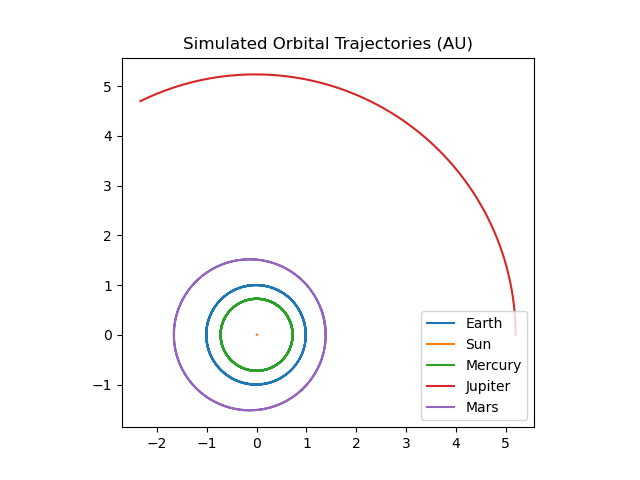
\includegraphics[width=\linewidth]{trajectory.png}
  \label{fig:trajectory}
\end{figure}





\end{document}
